\documentclass[11pt, a4paper]{report}

\usepackage[utf8]{inputenc}
\usepackage[T1]{fontenc}
\usepackage[french]{babel}

% Appel des packages dans le dossier preambule
\def\packagepath{../../../../../preambule}   % path du package princial

\usepackage{\packagepath/page_layout} % <--- Nouveau
\usepackage{\packagepath/config_info}
\usepackage{\packagepath/cadres_cours}
\usepackage{\packagepath/zones_reponse}
\usepackage{\packagepath/config_ds}
\usepackage{\packagepath/config_maths}

% --- PILOTAGE ---
%\def\visibleornot{visible}    % visible or invisible
\ifdefined\visibleornot\else\def\visibleornot{visible}\fi


\def\documentpath{./Sources_Latex}
\graphicspath{{./Images/}}


\def\ptsexoA{0}



\begin{document}

\def\level{Premiere}  % Classe à droite
\def\course{NSI}
\def\chaptername{Les tris} % Titre au centre
\def\docname{AP08~--~TD 1}        % Identifiant à gauche

\pagestyle{DS_LP}

\NomPrenom{}

\begin{exercice_cours}[Tri par sélection]{}

    \begin{enumerate}
        \item     Illustrer l'action du tri par sélection sur le tableau suivante: \verb|T=[17,12,25,43,16,17,34]|
        \item Réécrire la fonction \verb|tri_selection| du cours pour trier selon l'ordre décroissante.
        \item Indiquer quel est l'invariant de boucle de cet algorithme.
        \item Indiquer quelle est la complexité de cet algorithme.
    \end{enumerate}
\end{exercice_cours}

\begin{exercice_cours}[Tri par insertion]{}

    \begin{enumerate}
        \item     Illustrer l'action du tri par insertion sur le tableau suivante: \verb|T=[31,41,59,26,41,58,26]|
        \item Réécrire la fonction \verb|tri_insertion| du cours pour trier selon l'ordre décroissante.
        \item Indiquer quel est l'invariant de boucle de cet algorithme.
        \item Indiquer quelle est la complexité de cet algorithme.
    \end{enumerate}
\end{exercice_cours}


\begin{exercice_cours}[Tri par insertion]{}
    
    \begin{CodePythontexAlt}[TaillePolice=\normalsize, Largeur=1\linewidth,Centre,PremLigne=1, Lignes=false,]{}
fonction tri insertion naif(T)
    n <- ............
        pour i allant de 2 à n
            temp <- T[i]
            p <- 1
            tant que ...... < temp
                p <- p + 1
            fin tant que
            pour j allant de i-1 à p en decroissant
                T[j+1] <- ......
            fin pour
            T[p] <- ......
        fin pour
        renvoyer T
    fin fonction
\end{CodePythontexAlt}

    \begin{enumerate}
        \item expliquer pourquoi cet algorithme est un algorithme de tri par insertion
        \item A quoi correspodent les variables \verb|i| et \verb|p| dans cet algorithme ?
        \item Placer ces deux variables dans le schéma ci-dessous:
        
        \begin{center}
        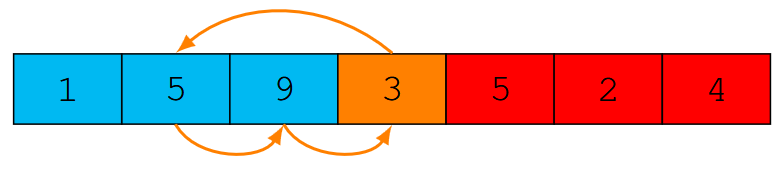
\includegraphics[width = 0.5\linewidth]{2026-06-08 20_47_05-Tris — Mozilla Firefox.png}
        \end{center}
        \item Déterminer la complexité de cet algorithme.
        \item Pourquoi cet algorithme est-il moins bon que celui vu en classe?
    \end{enumerate}

\end{exercice_cours}

\end{document}